\chapter{Overenie riešenia} \label{chapter:verification}
Funkčnosť a efektivitu riešenia v súlade s kladenými požiadavkami overíme v rozličných scenároch. Zároveň experimentálne
demonštrujeme odvodenie hyperparametrov klasifikácie špičiek s mriežkovým vyhľadávaním (grid search)
a vyjadríme úspešnosť zaužívanými metrikami.

\section{Pamäťová efektivita}
Skompilovaný program senzorovej jednotky sa zmestí do pamäte inštrukcií so značnou rezervou. Kódový segment zaberá
64,42\% alebo 81,8 kB dostupného priestoru vynímajúc vyhradené časti na vektory prerušení a vyrovnávacie pamäte procesora.
Obsadením 43,4 kB v segmente .bss, prevažne na staticky alokované polia reťazcov odosielaných správ, a nárokovania si 14,7 kB
konštánt, zostáva 82,3\% DRAM na haldu. Spotrebu SRAM v bajtoch podľa segmentov objektového súboru podľa nástroja
\emph{GNU size} uvádza tabuľka \ref{tab:ram-segments}.
\begin{table}[h]
\def\arraystretch{1.25}
\begin{tabular}{|l|llll|lll|}
\hline
                     & \multicolumn{4}{c|}{\textbf{IRAM (192 kB)}}                                                                              & \multicolumn{3}{c|}{\textbf{DRAM (328 kB)}}                                           \\ \hline
\textbf{Sekcia}      & \multicolumn{1}{l|}{CPU cache} & \multicolumn{1}{l|}{.vectors} & \multicolumn{1}{l|}{.text} & voľné                      & \multicolumn{1}{l|}{.bss}  & \multicolumn{1}{l|}{.data} & voľné (heap)                \\ \hline
\textbf{Veľkosť} & \multicolumn{1}{r|}{65536}     & \multicolumn{1}{r|}{1027}     & \multicolumn{1}{r|}{83780} & \multicolumn{1}{r|}{46265} & \multicolumn{1}{r|}{44392} & \multicolumn{1}{r|}{15040} & \multicolumn{1}{r|}{276440} \\ \hline
\end{tabular}
\caption{Rozdelenie pamäte v bajtoch medzi sekcie}
\label{tab:ram-segments}
\end{table}

Vyťaženie dynamickej pamäte z haldy lineárne závisí od počtu súčasne vyhodnocovaných údajových bodov. Trend sa prejavuje v grafe
celkovej percentuálnej naplnenosti haldy \ref{graph:mem-usage}. Markantný stály podiel z voľného priestoru až okolo 55 kB sa poskytne na komunikáciu cez WiFi a na TCP/IP protokolový zásobník (graf \ref{graph:task-memory})

Zvyšok majú k dispozícii vlákna úloh na manipuláciu so vzorkami osí zrýchlenia (x, y, z), na zdieľané koeficienty FFT a
konvolučné masky a  relatívne nepatrne si obsadia úlohy vzorkovania (imu) a zápisu na pamäťovú kartu (logger).
FreeRTOS je nastavený na dynamickú alokáciu zásobníkov, preto už pri veľkosti okna 8 potrebuje spracovateľská úloha 10 kB. Najdlhšie
akceptovateľné posuvné okno a tým aj veľkosť frekvenčnej transformácie je 1024 bodov, ktoré vzhľadom na 97\% spotreby haldy za istých
okolností vykazuje nestabilitu systému. Odporúča sa pri zložitejšom procese úpravy signálu vystačiť si s 512 bodmi.

\begin{figure}[h]
	\centering
     \hfill
     \begin{subfigure}{0.48\textwidth}
        \centering
     	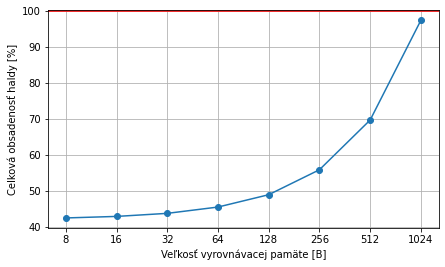
\includegraphics[width=\textwidth]{figures/verification/memory-usage-percentage.png}
     	 \caption{Celková spotreba pamäte}
     	 \label{graph:mem-usage}
     \end{subfigure}
     \hfill
      \begin{subfigure}{0.48\textwidth}
    	\centering
        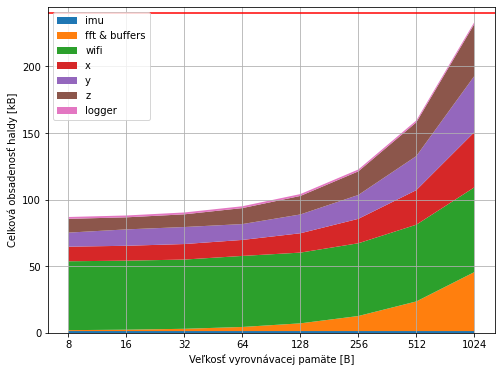
\includegraphics[width=\textwidth]{figures/verification/memory-profile-bytes.png}
         \caption{Rozdelenie pamäte medzi úlohy}
        \label{graph:task-memory}
     \end{subfigure}
     \caption{Profilovanie dynamickej pamäte z haldy v DRAM}
\end{figure}


Veľkosť vyrovnávacej pamäte má priamy dopad na objem posielanej sieťovej premávky, ako vyčísľuje tabuľka \ref{tab:msg-size} v bajtoch.
Sekvencia $n$ meraní má za následok $m$ frekvenčných vedierok s násobiacim faktorom veľkosti dátového typu. Nesúrodé
štruktúry sú vyjadrené úhrnnou mierou informácie.
\begin{table}[h]
\def\arraystretch{1.25}
\centering
\begin{tabular}{|l|r|r|rr|cr|r|l}
\cline{1-8}
\multirow{2}{*}{\textbf{MQTT topic}} & \multicolumn{1}{c|}{\multirow{2}{*}{\textbf{\begin{tabular}[c]{@{}c@{}}Min. \\topic \end{tabular}}}} & \multicolumn{1}{c|}{\multirow{2}{*}{\textbf{\begin{tabular}[c]{@{}c@{}}Veľkosť\\ v RAM\end{tabular}}}} & \multicolumn{2}{l|}{\textbf{Hlavička (h)}}                      & \multicolumn{2}{l|}{\textbf{Prvok (p)}}                         & \multicolumn{1}{c|}{\multirow{2}{*}{\textbf{\begin{tabular}[c]{@{}c@{}}Max. celková\\ veľkosť\end{tabular}}}} & \textbf{} \\ \cline{4-7}
                                     & \multicolumn{1}{c|}{}                                                                                     & \multicolumn{1}{c|}{}                                                                                  & \multicolumn{1}{c|}{\textbf{Min.}} & \multicolumn{1}{c|}{\textbf{Max.}} & \multicolumn{1}{c|}{\textbf{Min.}} & \multicolumn{1}{c|}{\textbf{Max.}} & \multicolumn{1}{c|}{}                                                                                         &           \\ \cline{1-8}
config/response                      & 21                                                                                                        & 124                                                                                                    & \multicolumn{2}{c|}{-}                                                  & \multicolumn{1}{r|}{-}             & \multicolumn{1}{l|}{}              & 450                                                                                                           &           \\ \cline{1-8}
samples                              & 13                                                                                                        & $4\cdot n$                                                                                                    & \multicolumn{1}{r|}{1}             & 3                                  & \multicolumn{2}{c|}{5}                                                  & $h + p\cdot n$                                                                                                      &           \\ \cline{1-8}
spectrum/+                           & 16                                                                                                        & $4\cdot m$                                                                                                & \multicolumn{1}{r|}{14}            & 22                                 & \multicolumn{2}{c|}{5}                                                  & $h + p\cdot m$                                                                                                 &           \\ \cline{1-8}
stats/+                              & 13                                                                                                        & 52                                                                                                     & \multicolumn{1}{r|}{4}             & 8                                  & \multicolumn{1}{r|}{9}             & 12                                 & 127                                                                                                           &           \\ \cline{1-8}
events/+                             & 14                                                                                                        & $20\cdot m$                                                                                               & \multicolumn{1}{r|}{18}            & 26                                 & \multicolumn{1}{r|}{17}            & 27                                 & $h + p\cdot m$                                                                                                &           \\ \cline{1-8}
\end{tabular}
\caption{Veľkosti Message Pack správ podľa MQTT topic}
\label{tab:msg-size}
\end{table}

Používaný formát Message Pack máp sa zväčša skladá z hlavičky, čo je názov
pre dvojice spoločne opisujúce variabilný počet obsiahnutých prvkov. Rozpätie v objeme hlavičky a položiek vyplýva z
balenia menších hodnôt pod kratšiu binárnu reprezentáciu. Produkovaný obsah sa rozčleňuje na základe logických kategórií
do MQTT topics vkladané do hlavičky protokolu s dĺžkou vyjadrenou vrátane najkratšieho prefixu.

Aby sme detekciou udalostí dosiahli úsporu v množstve prenášaných údajov, je žiaduce dosiahnuť kratšiu správu ako
zaslaním frekvenčných vedierok bez úpravy. Maximálna celková veľkosť dátovej nálože na tému \emph{events} musí byť menšia
ako na tému \emph{spectrum}. Pri $m = 16$ to činí 2 udalosti na okno (12,5\% z celkového počtu vedierok) a pri $m = 512$
sa musí vyskytnúť menej ako 93 udalostí na okno (18,16\%). Datasety z autobusov vykazujú emisiu udalostí najviac do
približne 6\% z úhrnného počtu frekvencií a 0,5\% v priemere. Štatistiky sa oplatí vytvárať pri najmenšom $n = 32$.

\begin{table}[h]
\def\arraystretch{1.25}
\centering
\begin{tabular}{|l|r|r|r|r|r|}
\hline
\textbf{Protokol}         & \textbf{Ethernet II} & \textbf{IPv4} & \textbf{TCP} & \textbf{MQTT}  & \textbf{Spolu}  \\ \hline
\textbf{Veľkosť hlavičky} & 14                   & 20            & 20           & \textgreater 5 & \textgreater 55 \\ \hline
\end{tabular}
\caption{Réžia sieťového prenosu v bajtoch}
\label{tab:net-overhead}
\end{table}

Vysielané správy zapúzdrené v sieťových protokoloch nižších vrstiev OSI modelu pridávajú
hlavičky na správne doručenie adresátovi, čím zvyšujú celkovú réžiu. V lokálnej WiFi sieti, kde bola infraštruktúra prítomná,
sa protokol MQTT pôsobiaci nad TCP, prenášal cez IPv4 v Ethernet-ových rámcoch. Každý paket má preto veľkosť vždy najmenej
podľa tabuľky \ref{tab:net-overhead}. Prenášaný obsah môže prevyšovať MTU, čo zapríčiní fragmentáciu do viacerých TCP segmentov
a ďalší nárast nadbytku.

\section{Časová efektivita}
Naplnenie kritérií na rýchlosť odozvy odmeriame systémovým časovačom s mikrosekundovou presnosťou.
Vplyv jednotlivých algoritmov na trvanie procesu úpravy signálu spriemerovaním 10 behov
je patrný z tabuľky \ref{tab:algorithm-execution}. Aktívna bola len úloha pre vybranú os zrýchlenia. S ohľadom na odchýlky
najmä v dôsledku prerušení od vzorkovania a obsluhy plánovača operačného systému sa potrebný čas navyšuje priamo úmerne
s dĺžkou postupnosti bodov.
\begin{table}[h]
\def\arraystretch{1.25}
\centering
\begin{tabular}{|l|l|l|l|l|l|l|}
\hline
\textbf{Veľkosť okna}         & \textbf{32} & \textbf{64} & \textbf{128} & \textbf{256} & \textbf{512} & \textbf{1024} \\ \hline
\textbf{Štatistiky bez korelácii}& 3673        & 7471        & 14652        & 29574        & 59158        & 112871        \\ \hline
\textbf{DFT}                     & 80          & 162         & 306          & 611          & 1243         & 2620          \\ \hline
\textbf{DCT}                     & 91          & 165         & 310          & 612          & 1226         & 2532          \\ \hline
\textbf{Špičky: susedia}         & 45          & 102         & 216          & 451          & 913          & 1812          \\ \hline
\textbf{Špičky: nulou do záporu} & 6           & 10          & 17           & 33           & 62           & 121           \\ \hline
\textbf{Špičky: horský turista}  & 19          & 32          & 54           & 109          & 199          & 431           \\ \hline
\textbf{Udalosti}                & 7           & 10          & 17           & 31           & 58           & 114           \\ \hline
\end{tabular}
\caption{Čas vykonávania algoritmov od veľkosti posuvného okna v $\mu s$ pri taktovacej frekvencii 160 MHz a intervale
plánovania 100 Hz}
\label{tab:algorithm-execution}
\end{table}

Výpočet štatistík sa najvýraznejšie podieľa na predlžovaní obratu spracovania rádovo v desiatkach
milisekúnd, zatiaľ čo väčšina krokov prebehne aspoň 40-krát rýchlejšie. Nevyrovnanosť zapríčiňujú miery vychádzajúce z
mediánu, pretože sa opakovane aplikuje Quickselect. Okrem toho si povšimneme, že v rýchlosti vykonávania nie je
žiaden rozdiel medzi frekvenčnou transformáciou s FFT a DCT, z dôvodu spomenutých nedostatkov knižničnej implementácie DCT-II.

Najpomalším hľadaním špičiek je metóda najvyššieho spomedzi susedov, ktorá má najhoršiu asymptotickú časovú zložitosť
spomedzi preberaných spôsobov. Dosahuje do 4-krát dlhšie časy ako algoritmus horského turistu a do 14-krát oproti prechodu
nulou do záporu. Výber prístupu ku klasifikácii špičiek nezáleží len od rýchlosti, ale tiež od charakteru rozloženia
vrcholov líšiaceho sa medzi algoritmami.

Vyhladzovanie v časovej alebo frekvenčnej doméne sa vyznačuje meniteľnou dĺžkou konvolučnej masky a počtom opakovaných
prechodov. Čas na dokončenie rovnako stúpa lineárne podľa oboch vlastností.
\begin{table}[h]
\def\arraystretch{1.25}
\centering
\begin{tabular}{|l|r|r|r|}
\hline
\textbf{Veľkosť masky}  & \textbf{4} & \textbf{16} & \textbf{64} \\ \hline
\textbf{1x} & 108        & 262         & 891         \\ \hline
\textbf{4x} & 413        & 1041        & 3697        \\ \hline
\textbf{8x} & 819        & 2065        & 7209        \\ \hline
\end{tabular}
\caption{Čas v $\mu s$ na vyhladzovanie v závislosti od veľkosti konvolučného jadra pri N = 512 a počtu opakovaní}
\label{tab:kernel-execution}
\end{table}

Porovnávanie variant fáz spracovania separátne nezohľadňuje serializáciu a publikovanie správ zvolených tém, či
dopad plánovania a synchronizácie na konkurentné úlohy. Pozrieme sa na výkonnosť postupu spracovania dát v dvoch odlišných prípadoch
pri frekvencii procesora 160 MHz a spriemerovaním desiatich spustení.

Správanie zariadenia v pokoji, bez odvodzovania akýchkoľvek štatistík, netvoriace sieťovú premávku, približuje tabuľka
\ref{tab:pipeline-simple}. Časy po pridaní výpočtu dostupných štatistík vrátane korelácií a upozorňovanie na udalosti
cez bezdrôtovú linku s RSSI na hladine cca -40 dBm popisuje tabuľka \ref{tab:pipeline-complex}. Vyhodnocuje sa trvanie behu
v mikrosekundách vzhľadom na veľkosť posuvného okna podľa algoritmu na hľadanie špičiek (číslovanie: A1, A2, A3, podľa kapitoly analýzy)
pre aktivovaný počet rozmerov akcelerácie. U troch dimenzií sa zohľadní do priemeru úloha s najdlhším časom vykonávania.
Frekvenčná transformácia je použitá za každej situácie FFT.

\begin{table*}[h]
     \def\arraystretch{1.25}
	 \centering
     \captionsetup[subtable]{position=below}

     \begin{subtable}{0.48\linewidth}
         \centering
		\begin{tabular}{|l|l|r|r|r|}
		\hline
		\textbf{}                       & \textbf{N}  & \textbf{32} & \textbf{256} & \textbf{1024} \\ \hline
		\multirow{3}{*}{\textbf{1 os}}  & \textbf{A1} & 518         & 2616         & 6401          \\ \cline{2-5}
 		                                & \textbf{A2} & 435         & 1598         & 6209          \\ \cline{2-5}
                                        & \textbf{A3} & 467         & 1695         & 3864          \\ \hline
		\multirow{3}{*}{\textbf{3 osi}} & \textbf{A1} & 2503        & 3077         & 10177         \\ \cline{2-5}
                                        & \textbf{A2} & 556         & 3340         & 10334         \\ \cline{2-5}
                                        & \textbf{A3} & 591         & 1295         & 4670          \\ \hline
		\end{tabular}
		\caption{V pokoji bez posielania správ}
		\label{tab:pipeline-simple}
	\end{subtable}
    \hfill
    \begin{subtable}{0.48\linewidth}
         \centering
		\begin{tabular}{|l|l|r|r|r|}
		\hline
		\textbf{}                       & \textbf{N}  & \textbf{32} & \textbf{256} & \textbf{1024} \\ \hline
		\multirow{3}{*}{\textbf{1 os}}  & \textbf{A1} & 14750       & 34883        & 129190        \\ \cline{2-5}
                              			& \textbf{A2} & 8824        & 34351        & 139451        \\ \cline{2-5}
                                        & \textbf{A3} & 13795       & 34890        & 137346        \\ \hline
		\multirow{3}{*}{\textbf{3 osi}} & \textbf{A1} & 23851       & 101978       & 273696        \\ \cline{2-5}
                                        & \textbf{A2} & 22981       & 78972        & 272161        \\ \cline{2-5}
                                        & \textbf{A3} & 24232       & 100156       & 270110        \\ \hline
		\end{tabular}
		\caption{Štatistiky s koreláciami a udalosti}
		\label{tab:pipeline-complex}
	\end{subtable}

	 \captionsetup[table]{position=below}
     \caption{Čas na spracovanie okna vzoriek v $\mu s$.}
     \label{tab:pipeline}
\end{table*}


Hraničný čas $t$ pokiaľ si vystačíme s tzv. ,,double buffering'', čiže sa neoneskorujeme od prúdu prichádzajúcich vzoriek o viac ako jednu
dĺžku vyrovnávacej pamäte $N$ nastáva, keď platí: $t \leq N / f_s$. Na určenie teoreticky najvyššej vzorkovacej frekvencie
pri danej dĺžke $N$ vezmeme časový parameter z tabuľky \ref{tab:pipeline}.

Ľubovoľné nastavenie spracovania signálu zvládne za okolností podľa \ref{tab:pipeline-simple} $f_s =$ 61,8 kHz pre jednorozmernú
sekvenciu a $f_s =$ 12,8 kHz pre trojrozmernú. Posielanie štatistík a udalostí z \ref{tab:pipeline-complex} pri jednej osi
dovoľuje $f_s =$ 2,1 KHz, ale pri väčších $N$ sa $f_s$ pohybuje nad 7 kHz. Tri dimenzie v tejto náročnej konfigurácii stíhajú nanajvýš $f_s$
od 1,3 KHz ($N = 1024$) do 3,7 kHz ($N = 32$). Limit vzorkovacej frekvencie senzora na 952 Hz zaručuje, že bežné prevádzkové
situácie sa stíhajú uskutočniť pred naplnením následného posuvného okna.

\section{Úspešnosť detekcie špičiek}
Syntetický signál so známymi časovo-frekvenčné spektrom sa zložil zo sinusoíd s exponenciálnym nábehom a dobehom.
Očakávaná kvantita zlúčených tónov na základný úsek sa stanovila podľa frekvencie vzorkovania ovplyvňujúcej rozlišovaciu
schopnosť susediacich komponentov. Pri 238 Hz sa zmiešalo 8 rozdielnych frekvencií, pri 476 Hz je ich 16 a pri 952 Hz sa
ich rozmiestnilo 32. Pseudonáhodný generátor inicializovaný so semienkom 10 vytvoril trénovaciu množinu s trvaním 60 sekúnd
a vzápätí 20 sekundovú testovaciu množinu.

Prehľadávaním parametrov detekcie špičiek hrubou silou nad trénovacím signálom boli odhalené najlepšie hodnoty z preddefinovanej sady.
Na testovacom signále sa zistili relevantné metriky úspešnosti klasifikácie vrcholov makro-priemerovaním medzi posuvnými oknami
o veľkosti $n$. Signál nebol dodatočne filtrovaný. Obdržanie spektrálneho obsahu v decibeloch prebehlo cez FFT s Hannovou
oknovou funkciou a 50\%  prekryvom okien. Vyčíslené sú presnosti (tab. \ref{tab:accuracy}), senzitivita (tab. \ref{tab:sensitivity}) a chybovosť (tab. \ref{tab:error-rate}) detekčných stratégií v percentách.

\begin{table}[h]
\def\arraystretch{1.1}
\centering
\begin{tabular}{|c|ccc|ccc|ccc|}
\hline
                    & \multicolumn{3}{c|}{\textbf{Algoritmus 1}}                                           & \multicolumn{3}{c|}{\textbf{Algoritmus 2}}                                           & \multicolumn{3}{c|}{\textbf{Algoritmus 3}}                                           \\ \hline
\diagbox{$n$}{$f_s$} & \multicolumn{1}{c|}{\textbf{238}} & \multicolumn{1}{c|}{\textbf{476}} & \textbf{952} & \multicolumn{1}{c|}{\textbf{238}} & \multicolumn{1}{c|}{\textbf{476}} & \textbf{952} & \multicolumn{1}{c|}{\textbf{238}} & \multicolumn{1}{c|}{\textbf{476}} & \textbf{952} \\ \hline
\textbf{128}        & \multicolumn{1}{c|}{84.46}        & \multicolumn{1}{c|}{73.76}        & 59.49        & \multicolumn{1}{c|}{83.67}        & \multicolumn{1}{c|}{74.12}        & 54.96        & \multicolumn{1}{c|}{83.69}        & \multicolumn{1}{c|}{73.41}        & 51.87        \\ \hline
\textbf{256}        & \multicolumn{1}{c|}{91.19}        & \multicolumn{1}{c|}{85.41}        & 73.59        & \multicolumn{1}{c|}{90.63}        & \multicolumn{1}{c|}{84.39}        & 71.84        & \multicolumn{1}{c|}{91.30}        & \multicolumn{1}{c|}{84.78}        & 72.00        \\ \hline
\textbf{512}        & \multicolumn{1}{c|}{95.54}        & \multicolumn{1}{c|}{91.91}        & 85.19        & \multicolumn{1}{c|}{95.45}        & \multicolumn{1}{c|}{91.92}        & 84.05        & \multicolumn{1}{c|}{95.54}        & \multicolumn{1}{c|}{91.93}        & 85.05        \\ \hline
\end{tabular}
\caption{Percentuálna presnosť klasifikácie frekvenčných špičiek}
\label{tab:accuracy}
\end{table}

\begin{table}[h]
\def\arraystretch{1.1}
\centering
\begin{tabular}{|c|lll|lll|lll|}
\hline
                    & \multicolumn{3}{c|}{\textbf{Algoritmus 1}}                                                                & \multicolumn{3}{c|}{\textbf{Algoritmus 2}}                                                                & \multicolumn{3}{c|}{\textbf{Algoritmus 3}}                                                                \\ \hline
\diagbox{$n$}{$f_s$}  & \multicolumn{1}{c|}{\textbf{238}} & \multicolumn{1}{c|}{\textbf{476}} & \multicolumn{1}{c|}{\textbf{952}} & \multicolumn{1}{c|}{\textbf{238}} & \multicolumn{1}{c|}{\textbf{476}} & \multicolumn{1}{c|}{\textbf{952}} & \multicolumn{1}{c|}{\textbf{238}} & \multicolumn{1}{c|}{\textbf{476}} & \multicolumn{1}{c|}{\textbf{952}} \\ \hline
\textbf{128}        & \multicolumn{1}{l|}{23.77}        & \multicolumn{1}{l|}{35.52}        & 41.04                             & \multicolumn{1}{l|}{16.11}        & \multicolumn{1}{l|}{22.33}        & 21.94                             & \multicolumn{1}{l|}{9.65}         & \multicolumn{1}{l|}{14.58}        & 9.47                              \\ \hline
\textbf{256}        & \multicolumn{1}{l|}{10.62}        & \multicolumn{1}{l|}{27.42}        & 29.98                             & \multicolumn{1}{l|}{6.58}         & \multicolumn{1}{l|}{15.33}        & 28.03                             & \multicolumn{1}{l|}{13.26}        & \multicolumn{1}{l|}{11.88}        & 9.51                              \\ \hline
\textbf{512}        & \multicolumn{1}{l|}{12.08}        & \multicolumn{1}{l|}{14.52}        & 32.09                             & \multicolumn{1}{l|}{3.68}         & \multicolumn{1}{l|}{0.00}         & 17.13                             & \multicolumn{1}{l|}{2.35}         & \multicolumn{1}{l|}{1.80}         & 15.26                             \\ \hline
\end{tabular}
\caption{Percentuálna senzitivita (TPR) klasifikácie frekvenčných špičiek}
\label{tab:sensitivity}
\end{table}

\begin{table}[h]
\def\arraystretch{1.1}
\centering
\begin{tabular}{|c|lll|lll|lll|}
\hline
                    & \multicolumn{3}{c|}{\textbf{Algoritmus 1}}                                                                & \multicolumn{3}{c|}{\textbf{Algoritmus 2}}                                                                & \multicolumn{3}{c|}{\textbf{Algoritmus 3}}                                                                \\ \hline
\diagbox{$n$}{$f_s$} & \multicolumn{1}{c|}{\textbf{238}} & \multicolumn{1}{c|}{\textbf{476}} & \multicolumn{1}{c|}{\textbf{952}} & \multicolumn{1}{c|}{\textbf{238}} & \multicolumn{1}{c|}{\textbf{476}} & \multicolumn{1}{c|}{\textbf{952}} & \multicolumn{1}{c|}{\textbf{238}} & \multicolumn{1}{c|}{\textbf{476}} & \multicolumn{1}{c|}{\textbf{952}} \\ \hline
\textbf{128}        & \multicolumn{1}{l|}{3.67}         & \multicolumn{1}{l|}{11.31}        & 21.59                             & \multicolumn{1}{l|}{3.06}         & \multicolumn{1}{l|}{5.38}         & 11.38                             & \multicolumn{1}{l|}{1.75}         & \multicolumn{1}{l|}{3.36}         & 4.87                              \\ \hline
\textbf{256}        & \multicolumn{1}{l|}{1.08}         & \multicolumn{1}{l|}{4.10}         & 8.66                              & \multicolumn{1}{l|}{1.26}         & \multicolumn{1}{l|}{3.12}         & 10.33                             & \multicolumn{1}{l|}{1.19}         & \multicolumn{1}{l|}{1.97}         & 2.41                              \\ \hline
\textbf{512}        & \multicolumn{1}{l|}{5.27}         & \multicolumn{1}{l|}{1.30}         & 5.00                              & \multicolumn{1}{l|}{0.96}         & \multicolumn{1}{l|}{0.00}         & 3.48                              & \multicolumn{1}{l|}{0.96}         & \multicolumn{1}{l|}{0.15}         & 1.95                              \\ \hline
\end{tabular}
\caption{Percentuálna chybovosť (FPR) klasifikácie frekvenčných špičiek}
\label{tab:error-rate}
\end{table}
Platnosť získaných percentuálnych metrík v absolútnej škále a hyperparametrov sa vzťahuje výlučne na zvolenú techniku
syntézy signálového priebehu, a teda nevieme potvrdiť podobné výsledky pre reálnu prepravu. Napriek tomu môžeme
z pravidelných tendencií dedukovať, že pomerne vysoká presnosť cca 84\%, ktorá zachováva senzitivitu, a chybovosťou do 5\%
sa stabilne objavuje na diagonálach, kde $n$ je polovicou $f_s$. Vtedy nachádzame ideálny pomer medzi rozlíšením
v čase a frekvencii aj v spektrogramoch.

Veľmi nízka senzitivita nezriedka 10 - 30\% je dôsledkom nedokonalej spätnej rekonštrukcie spektrálneho profilu a exaktnou
lokalizáciou vrchola, čím sa sinusoidy môžu ocitnúť posunuté o pár frekvenčných vedierok vedľa v porovnaní s označením v datasete.
Malý počet význačných frekvencií spôsobuje, že na prejavenie sa efektu zdanlivého poklesu senzitivity stačí, keď sa
mierne zmení poloha jedinej.

Spektrogram \ref{fig:synthetic-spectrogram} znázorňuje na testovacích dátach schopnosť prúdového algoritmu na detekciu zmien
frekvencií sa vysporiadať s nesprávne identifikovanými špičkami. Na vizualizácii je patrné, že
registrovanie prvého vrchola na súvislom výstupku nastávalo oneskorene prekročením určitej amplitúdy.
Ostatné algoritmy sa prejavovali obdobne, najvýraznejšie rozdiely sú v rozmiestnení falošných vrcholov.

\begin{figure}[h]
	\centering
     \begin{subfigure}{\textwidth}
        \centering
     	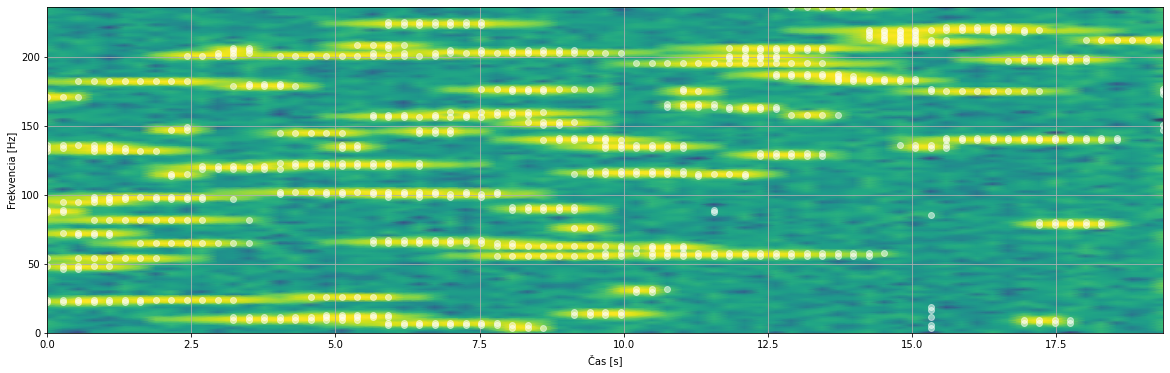
\includegraphics[width=\textwidth]{figures/verification/Sythetic-FFT-A1-476-256.png}
     	\caption{Nájdené špičky algoritmom č.1 v posuvných oknách vyznačené bielym kruhom}
     \end{subfigure}
     \begin{subfigure}{\textwidth}
    	\centering
    	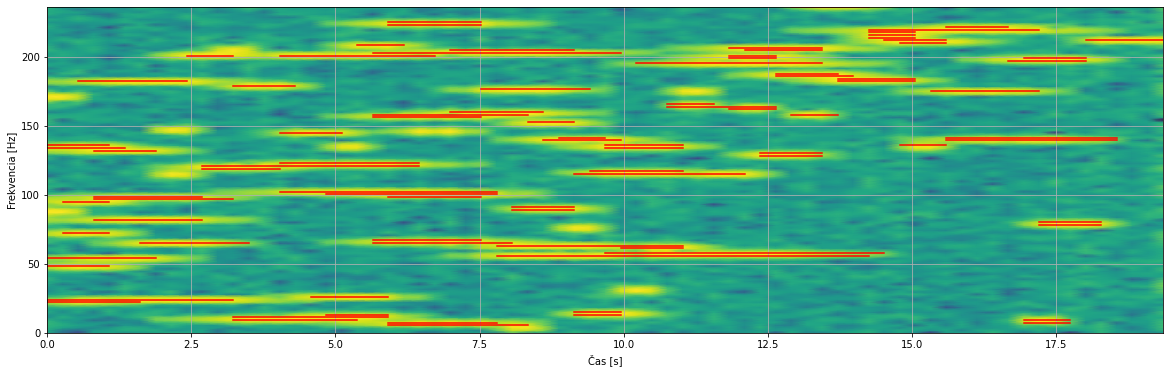
\includegraphics[width=\textwidth]{figures/verification/Sythetic-A1-events.png}
   		\caption{Zachytený priebeh udalostí frekvenčnej zmeny pri $t_{min} = 4$ a $t_{\Delta} = 1$}
     \end{subfigure}
     \caption{Spektrogramy detegovaných špičiek a udalostí pri $f_s = 476$ Hz a $N = 256$}
     \label{fig:synthetic-spectrogram}
\end{figure}

Parametre klasifikácie špičiek nájdené mriežkovým hľadaním, s ktorými sme dosiahli na konkrétnom syntetickom signále
najvyššie presnosti sú v tabuľke \ref{tab:grid-serach-parameters}.
\begin{table}[h]
\def\arraystretch{1.1}
\centering
\begin{tabular}{|c|c|ccc|cc|cccc|}
\hline
\multirow{2}{*}{\textbf{\begin{tabular}[c]{@{}c@{}}$f_s$\end{tabular}}} & \multirow{2}{*}{\textbf{\begin{tabular}[c]{@{}c@{}}$n$\end{tabular}}} & \multicolumn{3}{c|}{\textbf{\begin{tabular}[c]{@{}c@{}}Algoritmus 1\end{tabular}}} & \multicolumn{2}{c|}{\textbf{\begin{tabular}[c]{@{}c@{}}Algoritmus 2\end{tabular}}} & \multicolumn{4}{c|}{\textbf{\begin{tabular}[c]{@{}c@{}}Algoritmus 2\end{tabular}}}  \\ \cline{3-11}
                                                                                  &                                                                         & \multicolumn{1}{c|}{\hspace*{3mm}$k$\hspace*{3mm}}         & \multicolumn{1}{c|}{\hspace*{3mm}$\epsilon$\hspace*{3mm}}         & $h_{rel}$       & \multicolumn{1}{c|}{\hspace*{4mm} $k$ \hspace*{4mm}}                               &  $s$                              & \multicolumn{1}{c|}{$t$} & \multicolumn{1}{c|}{$h$} & \multicolumn{1}{c|}{$p$} & $i$ \\ \hline
238                                                                               & 128                                                                     & \multicolumn{1}{c|}{12}          & \multicolumn{1}{c|}{3}                  & 32                & \multicolumn{1}{c|}{2}                                 & 12                                & \multicolumn{1}{c|}{16}  & \multicolumn{1}{c|}{0}   & \multicolumn{1}{c|}{10}  & 8   \\ \hline
238                                                                               & 256                                                                     & \multicolumn{1}{c|}{3}           & \multicolumn{1}{c|}{1}                  & 32                & \multicolumn{1}{c|}{2}                                 & 16                                & \multicolumn{1}{c|}{16}  & \multicolumn{1}{c|}{0}   & \multicolumn{1}{c|}{10}  & 12  \\ \hline
238                                                                               & 512                                                                     & \multicolumn{1}{c|}{3}           & \multicolumn{1}{c|}{4}                  & 32                & \multicolumn{1}{c|}{2}                                 & 26                                & \multicolumn{1}{c|}{10}  & \multicolumn{1}{c|}{4}   & \multicolumn{1}{c|}{38}  & 0   \\ \hline
476                                                                               & 128                                                                     & \multicolumn{1}{c|}{3}           & \multicolumn{1}{c|}{4}                  & 16                & \multicolumn{1}{c|}{2}                                 & 9                                 & \multicolumn{1}{c|}{10}  & \multicolumn{1}{c|}{0}   & \multicolumn{1}{c|}{10}  & 0   \\ \hline
476                                                                               & 256                                                                     & \multicolumn{1}{c|}{12}          & \multicolumn{1}{c|}{4}                  & 32                & \multicolumn{1}{c|}{2}                                 & 12                                & \multicolumn{1}{c|}{16}  & \multicolumn{1}{c|}{0}   & \multicolumn{1}{c|}{10}  & 0   \\ \hline
476                                                                               & 512                                                                     & \multicolumn{1}{c|}{3}           & \multicolumn{1}{c|}{4}                  & 32                & \multicolumn{1}{c|}{1}                                 & 20                                & \multicolumn{1}{c|}{10}  & \multicolumn{1}{c|}{4}   & \multicolumn{1}{c|}{33}  & 0   \\ \hline
952                                                                               & 128                                                                     & \multicolumn{1}{c|}{3}           & \multicolumn{1}{c|}{4}                  & 0                 & \multicolumn{1}{c|}{2}                                 & 5                                 & \multicolumn{1}{c|}{10}  & \multicolumn{1}{c|}{0}   & \multicolumn{1}{c|}{10}  & 0   \\ \hline
952                                                                               & 256                                                                     & \multicolumn{1}{c|}{6}           & \multicolumn{1}{c|}{4}                  & 24                & \multicolumn{1}{c|}{2}                                 & 5                                 & \multicolumn{1}{c|}{16}  & \multicolumn{1}{c|}{0}   & \multicolumn{1}{c|}{10}  & 0   \\ \hline
952                                                                               & 512                                                                     & \multicolumn{1}{c|}{6}           & \multicolumn{1}{c|}{4}                  & 32                & \multicolumn{1}{c|}{2}                                 & 12                                & \multicolumn{1}{c|}{16}  & \multicolumn{1}{c|}{0}   & \multicolumn{1}{c|}{10}  & 0   \\ \hline
\end{tabular}
\caption{Parametre algoritmov detekcie špičiek na syntetických dátach (názvy sú skrátené na prvé písmená)}
\label{tab:grid-serach-parameters}
\end{table}

Manuálnym odladením parametrov na ukážkových záznamoch z vozidiel sme odskúšali rozdiely v schopnostiach algoritmov
na hľadanie špičiek povšimnúť si pretrvávajúce harmonické zložky. Výrez časovo-premenného spektra na obr. \ref{spectrum-slice}
s nájdenými špičkami zvýrazňuje prekážky správneho odlíšenia šumu alebo navzájom splývajúcich vrcholov. Niektoré lokálne extrémy
sú prehliadnuté pre nevýraznosť nad svojím okolím alebo pre prílišnú sploštenosť.
\begin{figure}[h]
   \centering
    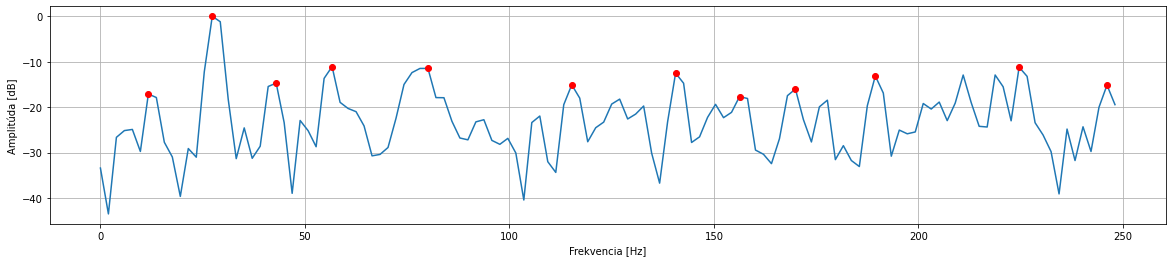
\includegraphics[width=\textwidth]{figures/verification/L83-slice-t-20-A1.png}
   \caption{Prierez spektrogramu okna 256 vzoriek s vrcholmi označenými algoritmom č.1
   v 20. sekunde záznamu \emph{L83\_4940\_Alexyho\_Svantnerova.csv}}
   \label{spectrum-slice}
\end{figure}

Nie je úplne zrejmé aké vodorovné konštelácie výrazných čŕt z obr. \ref{dataset-detection} sú korektne vyznačené,
a ktoré sú primerane agregované do spoločných udalostí. Podstatné frekvencie v stabilnej oblasti medzi časmi 22 a 33
sekundou ako napr. 11, 26, 56 Hz  boli univerzálne zaevidované. Detekcie z iného datasetu sú ilustrované v prílohe
\ref{appendix:spectrogram}.

\begin{figure}[h]
	\centering
     \begin{subfigure}{\textwidth}
        \centering
     	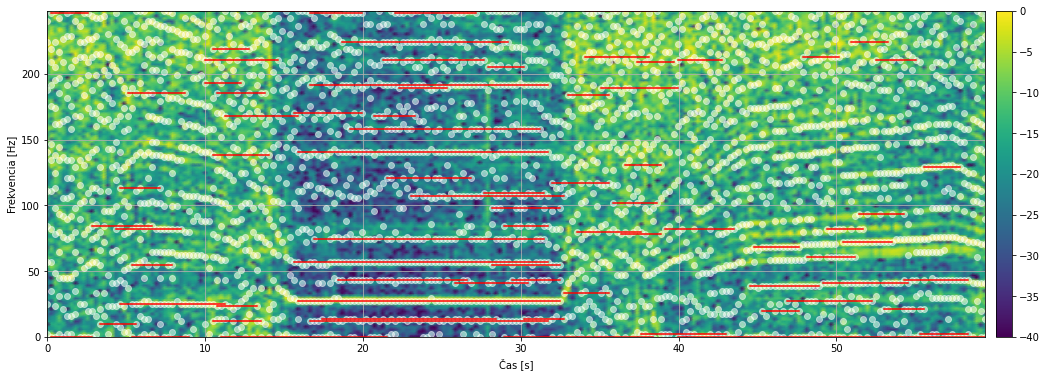
\includegraphics[width=\textwidth]{figures/verification/L83-dataset-A1.png}
     	\caption{Algoritmus č.1: $k = 5$, $\epsilon = 0$, $h_{rel} = 8$}
     \end{subfigure}
     \begin{subfigure}{\textwidth}
    	\centering
        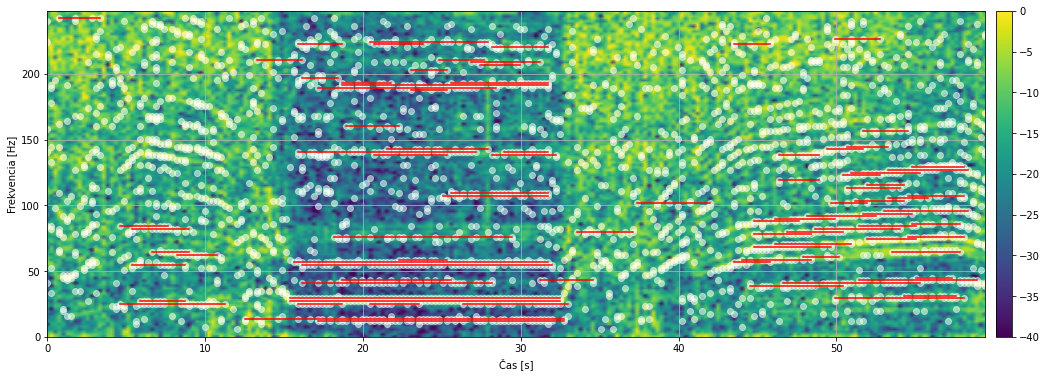
\includegraphics[width=\textwidth]{figures/verification/L83-dataset-A2.png}
        \caption{Algoritmus č.2: $k = 3$, $s = 7$}
     \end{subfigure}
      \begin{subfigure}{\textwidth}
    	\centering
        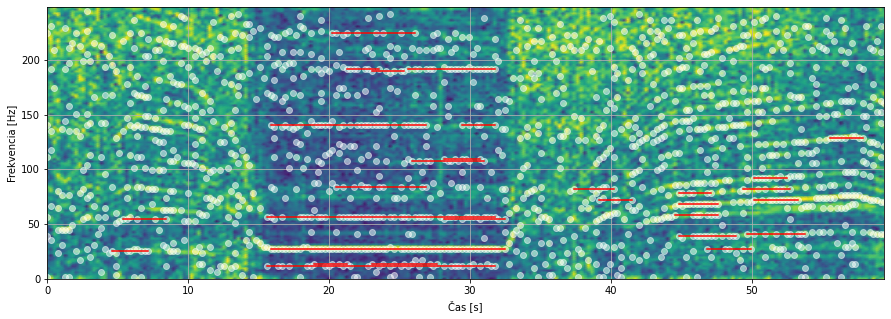
\includegraphics[width=\textwidth]{figures/verification/L83-dataset-A3.png}
        \caption{Algoritmus č.3: $t = 8$, $h = 1$, $p = 5$, $i = 0$}
     \end{subfigure}
     \caption{Detekcia udalostí v datasete \emph{L83\_4940\_Alexyho\_Svantnerova.csv} s $f_s = 500$ Hz, trvaním 60 s, dĺžkou okna 256,
     pri $t_{min} = 10$ a $t_{\Delta} = 4$}
     \label{dataset-detection}
\end{figure}
